
\documentclass[
    sigplan,
    10pt,
    review, % Note: remove the [review] option for the final document.
    natbib=false % Note: This ishere to be able to use Biber.
 ]{acmart}
\let\citename\relax

\settopmatter{printfolios=true,printccs=false,printacmref=false}

\acmConference[DLS'18]{Dynamic Languages Symposium}{November~6, 2018}{Boston, MA, USA}
\acmYear{2018}
\acmISBN{} % \acmISBN{978-x-xxxx-xxxx-x/YY/MM}
\acmDOI{} % \acmDOI{10.1145/nnnnnnn.nnnnnnn}
\startPage{1}

\setcopyright{none}

\bibliographystyle{ACM-Reference-Format}

\usepackage{booktabs}
\usepackage{subcaption}

\usepackage[
   backend=biber,
   bibencoding=utf8,
   style=alphabetic,
   hyperref=true,
   % citestyle=authoryear-comp,
   backref=false,
   sortlocale=en,
   url=true,
   doi=false,
   eprint=false
 ]{biblatex}
\addbibresource{biblio.bib}

\usepackage{minted}
\setminted{encoding=utf8}

\usepackage{tikz}
\usetikzlibrary{positioning}

\tikzset{
	box/.style = {
		draw = black,
        fill = white,
		rectangle,
		rounded corners = 2pt,
		text centered,
		minimum height = 5mm,
		minimum width = 10mm
	}
}

\usepackage{todonotes}
\newcommand\mb[1]{\todo[color=purple!20,size=\scriptsize]{#1}}
\newcommand\mbi[1]{\todo[color=purple!20,inline]{#1}}

\newcommand\ignore[1]{}

\begin{document}

\title{Relating an R Formalization to R} % I didn't thought much about this. Any suggestion?

\author{Martin Bodin}
\orcid{0000-0003-3588-3782}
\affiliation{
  %\position{}
  %\department{Department1}
  \institution{Center of Mathematical Modeling}
  \streetaddress{Beauchef 851}
  \city{Santiago}
  % \state{State1}
  % \postcode{Post-Code1}
  \country{Chile}
}
\email{mbodin@dim.uchile.cl}

\author{Tomás Diaz}
% \authornote{with author2 note}
% \orcid{nnnn-nnnn-nnnn-nnnn}
\affiliation{
  % \position{Position2a}
  \department{DCC}
  \institution{Universidad de Chile}
  \streetaddress{Beauchef 851}
  \city{Santiago}
  % \state{State2a}
  % \postcode{Post-Code2a}
  \country{Chile}
}
\email{tdiaz@dcc.uchile.cl}

\author{Éric Tanter}
% \authornote{with author2 note}
% \orcid{nnnn-nnnn-nnnn-nnnn}
\affiliation{
  % \position{Position2a}
  \department{DCC}
  \institution{Universidad de Chile}
  \streetaddress{Beauchef 851}
  \city{Santiago}
  % \state{State2a}
  % \postcode{Post-Code2a}
  \country{Chile}
}
\email{etanter@dcc.uchile.cl}

\begin{abstract}
Text of abstract \ldots.
\end{abstract}

% %% 2012 ACM Computing Classification System (CSS) concepts
% %% Generate at 'http://dl.acm.org/ccs/ccs.cfm'.
\begin{CCSXML}
  <ccs2012>
    <concept>
      <concept_id>10003752.10010124.10010131.10010133</concept_id>
      <concept_desc>Theory of computation~Denotational semantics</concept_desc>
      <concept_significance>500</concept_significance>
    </concept>
    <concept>
      <concept_id>10011007.10011006.10011066.10011070</concept_id>
      <concept_desc>Software and its engineering~Application specific development environments</concept_desc>
      <concept_significance>300</concept_significance>
    </concept>
    <concept>
      <concept_id>10011007.10011074.10011099.10011692</concept_id>
      <concept_desc>Software and its engineering~Formal software verification</concept_desc>
      <concept_significance>100</concept_significance>
    </concept>
  </ccs2012>
\end{CCSXML}

\ccsdesc[500]{Theory of computation~Denotational semantics}
\ccsdesc[300]{Software and its engineering~Application specific development environments}
\ccsdesc[100]{Software and its engineering~Formal software verification}
% %% End of generated code

\keywords{R, Coq, Formalization, Testing}

\maketitle

\section{Introduction}
\label{sec:intro}

% R is used a lot.
The R programming language~\parencite{R, ihaka1996r, Rwebsite}
has gotten a lot of attention in the recent years.
It is used in multiple fields (biology, finance, etc.),
and its community ranges over millions of users.
This diversity among R programmers
results in largely different programming styles.
The language itself is community driven and reflects this diversity.

% R is complex and we need to certify R softwares.
The R programming language is meant to be both expressive and powerful,
able to express complex notions in few keystrokes.
This sometimes comes with the cost of readability.
The semantics of R is subtle and contains numerous corner cases
which can be unexpected.
The reasons for these corner cases are numerous
and are often due to backward compatibility.
Another common reason is that R
is both used as a programming language and an interactive shell:
languages expectations are different in these two situations.

An example of such unexpected behaviors can be found
in R function calls.
There are many ways to call a function,
but to simplify\footnote{
    We here ignore the \mintinline{R}{...} notation
    as well as default arguments.
    They have non-trivial interactions with the calling methods
    described here.
} there are two ways to provide an argument:
either by position or by name.
In the example below, the first call to \mintinline{R}{f}
associates arguments by position, and the second by name.
These two associating ways can be mixed together in the same call.
%
Association by name can be made by prefix:
the third call associates \mintinline{R}{d} to \mintinline{R}{de}
because it is the only matching argument by prefix.
If more than one argument matches by prefix,
R rejects the call and throws an error,
as in the fifth call in the example below.
However, exact matches are not counted in this process:
in the fourth call below,
the name \mintinline{R}{ab} is an exact match
and thus only the argument \mintinline{R}{abc}
is left to be associated to \mintinline{R}{a},
leading to no error thrown.
\begin{minted}{R}
# The function f concatenates its 3 arguments.
f <- function (abc, ab, de) { c (abc, ab, de) }
# The next 4 calls below returns the same vector.
f (1, 2, 3) # Association by position.
f (de = 3, abc = 1, ab = 2) # By name.
f (1, d = 3, 2) # Mixed ways.
f (3, a = 1, ab = 2) # a is associated to abc.
# The next call to f throws an error.
f (a = 3, 1, 2) # Several prefixes.
\end{minted}

Such subtle behaviors are numerous in R~\parencite{RInferno}.
Debugging tools exist~\parencite{mcpherson2014},
but they can't always compensate R's complex semantics.
Consequently, bugs occurs in R programs
and fully trusting such programs can be difficult.

% We need a formalization of the language.
Formal methods offer a solution to this trust issue:
proof assistants such as Coq~\parencite{Coq} enable us
to formally prove program properties with a high amount of trust.
But to formally prove that an R program meets its specification,
we need a formal semantics of R.
In particular, we want to catch all the subtle cases of R semantics,
such as implicit type conversions.
These corner cases are indeed a typical place were bugs appears.
Such a semantics for the full language will inevitably be complex
because of the quantity of such cases.

% This formalization is quite large, and we need to certify it.
This opens a trust problem:
how can such a large semantics (and hence the proofs made from it)
can be trusted if it is that complex?
To be able to trust such a formalization,
we need to relate to the R reference interpreters, GNU~R~\parencite{Rwebsite}.
This relation between the formalism and trust sources
is not always considered to be an important part of the formalization process.
In practise however, it often requires a large amount of work
to be done properly~\parencite{leroy2014pip}.
Given the size of our formalization,
we consider this part to be the most important of our contributions.
Our code is available online at
\url{https://github.com/Mbodin/proveR/releases/tag/DLS2018}\todo{make this tag appear}.

% Contributions.
We introduce CoqR\mb{Are we fixed on the name?},
a formalization of the R programming language in the Coq proof assistant.
This is a continuation of a previous work~\parencite{CoqRCoqPL},
\mb{Political choice here: is it a good idea to cite this previous work?}
in which we formalised a small core of the R language.
The additional contribution of this paper is the additional
of a non-trivial quantity of R features,
which enabled us to import R libraries.
%
Our main contribution is to provide two methods to relate this formalization
to R reference interpreter, GNU~R.
First, our semantics has been written in a way mimicking GNU~R's source code.
Second, our semantics is executable and we have extensively tested it
against R reference interpreter.
%
This two-factors method is very close to the one of JSCert,
which we discuss in Section~\ref{sec:related:work}.

% Outlines.
This paper is organized as follows.
Section~\ref{sec:coq:interp} presents the Coq denotational semantics.
In particular, Section~\ref{sec:eyeball:closeness} presents
how this semantics is syntactically close to the C source code of R.
Section~\ref{sec:testing:architecture} then presents our testing architecture.
Not only this architecture is used as a way to relate our semantics
with R reference interpreter,
it also provided immediate benefits during the development of the semantics.
Section~\ref{sec:driving:development} presents these benefits.
The testing results are shown in Section~\ref{sec:test:results}.
Finally, Section~\ref{sec:proofs} presents some proofs that have been done
using our language formalization.

\section{Coq Interpreter}
\label{sec:coq:interp}

Our semantics of R is presented on the form of an interpreter.
Denotational semantics are usually not the best fit for Coq proofs---%
inductive operational semantics are usually more adapted---%
but it comes with a crucial advantage:
it can be run, and thus tested.
In this section, we show how we defined this interpreter.

\subsection{Eyeball Closeness}
\label{sec:eyeball:closeness}

\begin{figure*}
    \centering{}
\begin{subfigure}{.55\textwidth}
\begin{minted}{C}
EXP* do_attr (EXP* call, EXP* op, EXP* args, EXP* env){
  EXP* argList, ans, car;
  int nargs = R_length (args);
  argList = matchArgs (do_attr_formals, args, call);
  PROTECT (argList);
  if (nargs < 2 || nargs > 3)
    error ("Wrong argument count.");
  car = CAR (argList);
  /* ... */
  return ans;
}
\end{minted}
    \caption{original C function}
    \label{fig:c:do_attr}
\end{subfigure}
\begin{subfigure}{.44\textwidth}
\begin{minted}{Coq}
Definition do_attr S
    (call op args env : EXP_pointer) :=
  let%success nargs := R_length S args using S in
  let%success argList :=
    matchArgs S do_attr_formals args call using S in
  if nargs <? 2 || nargs >? 3 then
    result_error S "Wrong argument count."
  else
    read%list car, _, _ := argList using S in
    (* ... *)
    result_success S ans.
\end{minted}
    \caption{Coq translation}
    \label{fig:coq:do_attr}
\end{subfigure}
    \caption{Original C function and Coq translation of \mintinline{C}{do_attr}}
    \label{fig:do_attr}
\end{figure*}

One key specificity of this interpreter is that it has been designed
to be similar to the original C source code of GNU~R.
More precisely, they are related by a line-to-line correspondence
(also called \emph{eyeball closeness}):
every one or two lines of our interpreter
correspond to one or two lines of the reference interpreter.
%
This correspondence helped us during the development process:
whenever a bug was encountered during testing,
we would localize the line responsible for the difference in behavior
between GNU~R and CoqR,
then check the line-to-line correspondence.
Such checks were quick and easy to do,
and often lead to a quick fix of CoqR.
%
Figure~\ref{fig:do_attr} shows an example of such correspondence:
Figure~\ref{fig:c:do_attr} shows a C function,
and Figure~\ref{fig:coq:do_attr} its Coq translation.

Coq and C are widely different programming languages:
Coq is purely functional
whilst global side-effects appear frequently in C code.
Furthermore, Coq is designed to reject any function
whose behavior is not entirely defined
(it is for instance impossible to miss a case in a pattern matching),
whilst undefined behaviors are accepted by C compilers.
Finally, Coq functions are guaranteed not to loop,
whilst non-termination is not an issue in C.
%
To make Coq functions follow C paradigms,
we thus introduced a state, error, and fuel monad, shown below.
\begin{minted}{Coq}
Inductive result (A : Type) :=
  | result_success : state -> A -> result A
  | result_error : state -> string -> result A
  | result_longjump : state -> context -> result A
  | result_impossible : state -> string -> result A
  | result_not_implemented : string -> result A
  | result_bottom : state -> result A.
\end{minted}
The main constructor is \mintinline{Coq}{result_success}:
it is returned when a computation was successful.
In addition to the result (of type \mintinline{Coq}{A} in the definition),
it carries the global state.
%
The constructor \mintinline{Coq}{result_error} is meant to catch
errors thrown by GNU~R,
for instance a type-error when calling a non-function:
these errors are not catchable and immediately ends the execution.
A \mintinline{Coq}{string} is provided to help our debugging process.
%
Some specific calls in GNU~R source code require
the \mintinline{Coq}{result_longjump} constructor:
it typically appears in constructs like \mintinline{R}{break}
or \mintinline{R}{return} and involves a non-local jump in C.
We won't give much details about this constructor in this paper.
%
Unspecified C behaviors are translated into \mintinline{Coq}{result_impossible}.
This typically includes dereferencing an invalid pointer.
Getting this result immediately ends the Coq interpreter:
it is meant to be unreachable.
%
Given the size of the interpreter,
it was important to be able to execute it without it being complete.
The \mintinline{Coq}{result_not_implemented} is thus important
for the development, and is treated specifically in our testing framework.
%
Finally, \mintinline{Coq}{result_bottom} is returned
to end the execution when reaching the maximum number of executed instructions
(also called \emph{fuel}).
This is meant to artificially make our interpreter terminate,
despite the fact that the executed R program may not.

This monad is associated with a monadic binder,
written \mintinline{Coq}{let%success}.
It expects its argument to be of the form
\mintinline{Coq}{result_success}
to name the carried result in the following code,
the state being propagated.
All other kinds of results are propagated.
It is typically used when calling a function:
in Figure~\ref{fig:coq:do_attr},
the calls to \mintinline{Coq}{R_length}
and \mintinline{Coq}{matchArgs}
may return an unsuccessful result,
but the code that follows will only be executed if the result is successful.
%
This monadic interpreter is similar the one of the JSExplain project~\parencite{JSExplain},
which aims at defining a JavaScript interpreter readable by non-specialists.
We believe this helps finding bugs in CoqR.

We now describe how we modelled GNU~R's heap.
Although the underlying language is C,
GNU~R has been designed with a specific structure in mind~\parencite{R}.
Almost all objects manipulated by the GNU~R interpreter
are called \emph{basic language elements}---or \mintinline{C}{EXP} in C.
Each of them are composed of a header and some information depending
of the basic language elements.
%
The header stores the type of the basic language element,
a list of attributes,
as well as several mostly-boolean informations
(for instance whether it can be updated in place
without breaking other places of the heap).
% For instance, the header of an environment stores whether
% the environment is locked,
% which prevents the addition or removal of its bindings.
There are 24 different types of basic language elements in R,
9 of which being different kinds of vectors.
%
What comes afterwards depends on the type.
For instance, lists contains three pointers:
one to the first element (named \mintinline{Coq}{car}),
to the following of the list (\mintinline{Coq}{cdr}),
and to an optional name for the first element (\mintinline{Coq}{tag}).
Vectors types store their length,
followed in memory by a C array.
The size of this array depends both of its length
and the size of the stored data.
Figure~\ref{fig:basic:language:elements} illustrates this
with integer and complex vectors (which are composed of two floats).
%
Needless to say that the way memory is used in C
makes it easy to unguardedly access a cell out of bounds,
which would lead to an undefined behavior.

\begin{figure}
    \centering{}
    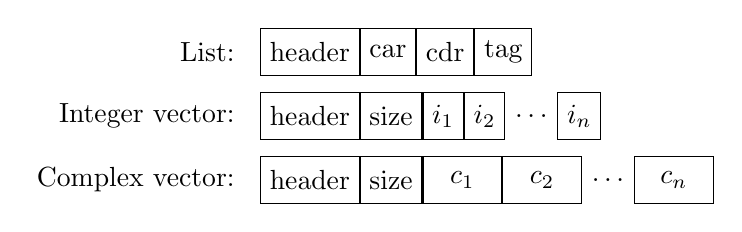
\begin{tikzpicture}
        \node [draw = black, rectangle, minimum height = 6mm, anchor = base] (hlist) {header} ;
        \node [draw = black, rectangle, minimum height = 6mm, anchor = base, right = 0pt of hlist] (car) {car} ;
        \node [draw = black, rectangle, minimum height = 6mm, anchor = base, right = 0pt of car] (cdr) {cdr} ;
        \node [draw = black, rectangle, minimum height = 6mm, anchor = base, right = 0pt of cdr] (tag) {tag} ;
        \node [left = 2mm of hlist] (nlist) {List:} ;

        \node [draw = black, rectangle, minimum height = 6mm, anchor = base, below = 2mm of hlist] (hvector1) {header} ;
        \node [draw = black, rectangle, minimum height = 6mm, anchor = base, right = 0pt of hvector1] (size1) {size} ;
        \node [draw = black, rectangle, minimum height = 6mm, anchor = base, right = 0pt of size1] (i1) {\(i_1\)} ;
        \node [draw = black, rectangle, minimum height = 6mm, anchor = base, right = 0pt of i1] (i2) {\(i_2\)} ;
        \node [anchor = base, right = 0pt of i2] (i3) {\(\ldots\)} ;
        \node [draw = black, rectangle, minimum height = 6mm, anchor = base, right = 0pt of i3] (in) {\(i_n\)} ;
        \node [left = 2mm of hvector1] (nvector1) {Integer vector:} ;

        \node [draw = black, rectangle, minimum height = 6mm, anchor = base, below = 2mm of hvector1] (hvector2) {header} ;
        \node [draw = black, rectangle, minimum height = 6mm, anchor = base, right = 0pt of hvector2] (size2) {size} ;
        \node [draw = black, rectangle, minimum height = 6mm, minimum width = 1cm, anchor = base, right = 0pt of size2] (c1) {\(c_1\)} ;
        \node [draw = black, rectangle, minimum height = 6mm, minimum width = 1cm, anchor = base, right = 0pt of c1] (c2) {\(c_2\)} ;
        \node [anchor = base, right = 0pt of c2] (c3) {\(\ldots\)} ;
        \node [draw = black, rectangle, minimum height = 6mm, minimum width = 1cm, anchor = base, right = 0pt of c3] (cn) {\(c_n\)} ;
        \node [left = 2mm of hvector2] (nvector2) {Complex vector:} ;
    \end{tikzpicture}
    \caption{Basic language elements in memory}
    \label{fig:basic:language:elements}
\end{figure}

This is an issue,
as we can't directly translate unguarded C accesses into Coq.
We thus need a model of the heap in Coq.
Figure~\ref{fig:EXP} shows how we defined \mintinline{Coq}{EXP}
in Coq.
Basic language elements are records storing a header
and data,
which is defined as a sum-type of all its combinations.
For instance, lists are defined by three pointers.
Vectors are records storing their length and a list:
in Coq, the data of vector is stored directly in the \mintinline{Coq}{EXP} structure
and not following it in memory as in C.

\begin{figure}
\begin{minted}{Coq}
Record ListStruct := make_ListStruct {
    lSist_carval : EXP_pointer ;
    lSist_cdrval : EXP_pointer ;
    lSist_tagval : EXP_pointer
  }.

Record Vector_EXP (A : Type) := make_Vector_EXP {
    Vector_length : nat ;
    Vector_data :> list A
  }.

Inductive EXPData :=
  | listExp : ListStruct -> EXPData
  | envExp : EnvStruct -> EXPData
  | EXP_VectorInteger : Vector_EXP int -> EXPData
  | EXP_VectorComplex : Vector_EXP complex -> EXPData
  (* ... *).
Coercion listExp : ListStruct >-> EXPData.
Coercion envExp : EnvStruct >-> EXPData.
(* ... *)

Record EXP := make_EXP {
    EXP_header :> EXPHeader ;
    EXP_data :> EXPdata
  }.
\end{minted}
    \caption{Basic language elements (\mintinline{C}{EXP}) in Coq}
    \label{fig:EXP}
\end{figure}

To ease readability, coercions have been used extensively.
Coercions is a mechanism to mark some constructors as implicit.
For instance, if Coq expects a \mintinline{Coq}{EXPData}
and is given a \mintinline{Coq}{ListStruct},
then the constructor \mintinline{Coq}{listExp} will be implicitly called.
In the context of CoqR,
this is more than a simple syntactic notation:
it helps the line-to-line correspondence
by erasing in the code things that are not present in C.
Indeed, if one points to either a list or an environment in C,
the notation to access its list or its environment is the same.
%
Of course, this implicit notation is only one-way:
given a \mintinline{Coq}{ListStruct},
we can convert it into an \mintinline{Coq}{EXPData},
but to perform the converse, we have to pattern match
on the shape of the \mintinline{Coq}{EXPData}.
%
This pattern matching is performed through specific monadic binders.
For instance in Figure~\ref{fig:coq:do_attr}, \mintinline{Coq}{read%list}
gets the \mintinline{Coq}{EXP} stored in the state \mintinline{Coq}{S}
and pointed by \mintinline{Coq}{argList},
then pattern-matches it as a list,
extracting the \mintinline{Coq}{car}, \mintinline{Coq}{cdr},
and \mintinline{Coq}{tag} fields.
If the pointer is not in the domain of the state \mintinline{Coq}{S}
or if the associated \mintinline{Coq}{EXP} object is not a list,
then \mintinline{Coq}{result_impossible} is returned:
this would correspond to an undefined behavior in C
(dereferencing an invalid pointer or accessing the wrong projection of a \mintinline{C}{union}).
The accesses in Coq are thus guarded by a monadic binder,
whilst mimicking the unguarded accesses of C.

In Figure~\ref{fig:c:do_attr}, the \mintinline{C}{PROTECT} macro
has been removed in the Coq translation of Figure~\ref{fig:coq:do_attr}.
This macro is performing garbage collecting actions
(in this case, it saves the object \mintinline{C}{argList} from garbage collection),
and we chose not to model this part of GNU~R.
Indeed, garbage collection is not supposed to change the result of any computation.
Not modelling this part removed frequent lines in the translation process,
enabling anyone wanting to reuse our formalization to focus on the computational part.
%
At this stage, the reader should be able
to compare the C and Coq programs of Figure~\ref{fig:do_attr}
line by line.
The rest of CoqR was similarly defined.

\begin{figure*}
    \centering{}
\begin{subfigure}{.5\textwidth}
\begin{minted}{C}
  static EXP* formals = NULL;
  if (formals == NULL)
    formals = allocFormalsList2 (install ("x"),
                install ("which"));
\end{minted}
    \caption{C snippet}
    \label{fig:c:do_attr:formals}
\end{subfigure}
\begin{subfigure}{.49\textwidth}
\begin{minted}{Coq}
Definition do_attr_init globals runs S :=
  let%success x :=
    install globals runs S "x" using S in
  let%success which :=
    install globals runs S "which" using S in
  allocFormalsList2 globals S x which.
\end{minted}
    \caption{Coq translation}
    \label{fig:coq:do_attr:formals}
\end{subfigure}
    \caption{Another snippet of \mintinline{C}{do_attr} and its Coq translation}
    \label{fig:do_attr:formals}
\end{figure*}

\subsection{Structure of the Interpreter}
\label{sec:coq:structure}

Size of the project.
How we cope to this size.

The [runs] trick to support looping in Coq in a structured way (similar to JSRef).

Definition of the core and of the features.

Initialization of R, global variables.

Ignored aspects.
As stated in Section~\ref{sec:eyeball:closeness},
we did not modelled the garbage collector.

\subsection{Shim}
\label{sec:shim}

Issues with parsing.
How the parser itself is in a one-to-one correspondence with the original R parser.
Why this still doesn't prevent us from difference in behavior.


\section{Testing Architecture}
\label{sec:testing:architecture}

Two goals.
First providing trust to the formalization by certifying the absence of bugs.
Second, help the development of the formalization by catching bugs early.

\subsection{Methodology}
\label{sec:test:methodology}

Various kinds of tests (multiline, line-by-line, tests that are expected to fail, etc.).

What is considered to be a failure.

\subsection{Base Library}
\label{sec:library}

Prior to execute any expression, GNU~R performs a lot of actions.
First, the heap is initialised.
This process involves initialising most global variables.
Then, GNU~R executes the base library.
It is a group of files written in R,
totalizing 19,000 lines of code.
%
This means that we have to be able to run the base library
to correctly test our interpreter.
For instance, without the base library,
no variable named \mintinline{R}{T} is defined:
running the program \mintinline{R}{T} results in a lookup error
in our interpreter whilst resulting in \mintinline{R}{TRUE} in R.
After running the base library,
which includes a line of the form \mintinline{R}{T <- TRUE},
our interpreter behaves as R on this same program.

Most of these functions are just links to internal functions
with some argument checking or default argument.
Below is an example:
the defined function \mintinline{R}{which} behaves very similarly
to the internal \mintinline{R}{which} function.
The difference is that \mintinline{R}{which} takes two additional
optional parameters.
With their default values, the behaviour of this function
is the same as the corresponding internal function:
this definition extends the original simpler behaviour of the function.
\begin{minted}{R}
which <- function (x, arr = FALSE, names = TRUE) {
    wh <- .Internal (which (x))
    if (arr && !is.null (d <- dim (x)))
        array (wh, d, dimnames (x), names = names)
    else wh
}
\end{minted}

These functions are easily run:
only the \mintinline{R}{function} keyword is necessary
to define the function \mintinline{R}{which}.
Of course, once the base library run,
if one actually calls the function \mintinline{R}{which},
a not-implemented exception will be thrown:
the internal function \mintinline{R}{function (x) .Internal (which (x))}
has not been implemented.
%
\todo{What follows is to be entirely rewritten, I'm afraid.}
We consider that this behavior is expected:
the main reason to run the base library is to correctly
classify the results of our interpreter.
For instance, the difference of behavior of the program \mintinline{R}{T}
before and after running the base library is problematical:
the reason our interpreter would fail in this program without the base library
is not due to our interpreter itself, but because the base library is missing.
Classify the internal function \mintinline{R}{which} as being not implemented
is a correct classification for our interpreter.

The base library also prepares the base environment.
For instance, the file \texttt{constants.R} of the base library
contains the following line.
Such lines are more complex as they involve computations:
to be able to run the base library,
we need to implement the \mintinline{R}{atan} function---%
in this case, using an OCaml hook.
Other examples of R functions that had to be implemented
to run the base library include functions to create new environments,
logical operators,
the \mintinline{R}{substitute} function,
the \mintinline{R}{$} operator \ignore$% Added to help my TeX syntax coloration…
(which fetches an identifier in a named list or an environments),
as well as various internal functions.
\begin{minted}{R}
pi <- 4 * atan (1)
\end{minted}

We have been able to run the entire base library.
We believe that this is an evidence that we caught a sizeable
part of the language features.


\subsection{Driving the Development Process}
\label{sec:driving:development}

Identifying low-hanging fruits.

How the other results (Potential fail, Not implemented) helped the Coq development.

\subsection{Results}
\label{sec:test:results}

How much tests are passed and failed.
What does this mean (one line can trigger more than one pass).

Bugs found (and where).

We extended the testing framework during development by adding new kinds of recognised
data structure.
We consider that the amount of work to extend the framework in another direction
(thus reducing the number of Unknown) is sufficiently low.

\section{Proofs}
\label{sec:proofs}

Tactic development.
Given the size of the formalization, some of these proofs would never have been possible
without some proof automation.
Automation metric: size of the .vo / size of the .v.

Examples of properties that we have proven with our formalization.

Example of tactic in action:
computeR after an allocation updating all the \mintinline{Coq}{safe_pointer}, for instance.

\section{Related Work}
\label{sec:related:work}

R is a notably difficult programming language~\parencite{RInferno},
whose semantics is constantly moving---%
see for instance the recent addition
of R's alternative representation~\parencite{altrepR}.
In our formalization, we chose to ignore these fast moving parts,
but these parts are used by real-world R programs.
Furthermore, the diversity of R users is such that different R programs
will use very different libraries and features,
as the generally accepted guideline~\parencite{RGuidelines}
doesn't restrain users about them.
This makes tools difficult to build for R,
and as a consequence, relatively few tools for R exist
in comparison to the size of its community.

As a consequence,
there exist few testing framework in R.
The testR~\parencite{maj2013testr, 2014testr} project,
which later evolved into Genthat~\parencite{genthat} library,
is however based on an interesting way of generating unit tests for R functions.
It start from a program using the functions to be tested.
It then annotates and executes this program,
storing the trace of the calls to the functions to be tested.
Unit tests are then generated from this trace.
The Genthat library is thus useful to generate tests for a library
given some program using it,
which can then be used to ensure that further versions of the library
don't break already existing code.

GNU~R is not the only R interpreter that exist.
Many existing interpreters are based on the same C core code,
but use different libraries for linear algebra,
usually optimised for a given usage.
%
The FastR~\parencite{kalibera2014fast} project takes a different approach
as it also reimplemented the core code.
It is based on the Truffle~\parencite{wuerthingertruffle}
self-optimizing framework.
Their tool is faster than the reference interpreter
in the language interpretation, and not only the linear-algebraic part.
%
In both cases, a difference of behavior between GNU~R
and the specialized interpreter is considered as a bug.
We believe that this support our choice of strongly basing
our work on this interpreter.

To the extent of our knowledge,
we are the first to provide a mechanized specification of R.
But the general goal of formalizing full real-world languages---%
as opposed to small subsets---is not new.
%
JavaScript is a particular relevant example.
Indeed, empirical analyses~\parencite{RichardsHBV11}
have confirmed that the language features
that are usually ignored in the formalised subsets of R
are actually important for actual web developers.
%
In the case of JavaScript, there are several trust sources.
First, the language is precisely specified by the ECMAScript specification~\parencite{es2019}.
Second, there exist various test suites~\parencite{test262, mozillatests}
as well as several widely used interpreters.
As a consequence, various formal specifications of JavaScript exist,
each related with different of its trust sources.

The first full formal semantics~\parencite{aplas08}
is a semantics related to the third version of the ECMAScript specification.
It had a major influence on the definitions of further JavaScript formal
specification~\parencite{ses, popl14jscert, popl12-Towards, usenix}.
It served as the formal basis to prove the soundness of security-related
JavaScript subsets~\parencite{MMT-CSF-TR09, mmt-esorics09, mmt-oakland10}.
This work was however not mechanized, making it difficult to be used
as a basis for other formal works.

In parallel, several formal semantics~\parencite{js-ml, Guha2010, Politz:S5, kjs}
for JavaScript were based on a JavaScript interpreter.
These semantics are related to JavaScript test suites,
either by comparing the results with the expected result,
or by comparing results with widely used JavaScript interpreters.
These formalizations tend to be easier to build
as testing frameworks already exist.
Furthermore, they are usually easier to understand by non-specialists.
However, such formalizations suffer from all the issues of test suites:
in JavaScript, the \mintinline{javascript}{for}-\mintinline{javascript}{in}
feature was then loosely tested,
and its behavior varied from interpreters to interpreters.

The JSCert formalization~\parencite{popl14jscert}
is an interesting step forward as it was designed
to be related with both the ECMAScript specification and the JavaScript test suites.
The formalization is composed of two parts:
a mechanized specification and an interpreter.
The JSCert specification is syntactically related with the ECMAScript specification
and the interpreter passes its test suites.
The specification and the interpreter are related to each other by a Coq proof.
This double-relation provides a large amount of trust to JSCert.
In practice, both relations served to find issues in the JSCert specification,
but also some implementation bugs in other interpreters,
as well as mistakes in the ECMAScript specification.
Furthermore, JSCert is mechanized:
this facilitates its reuse for other projects.
However, this project involved 8 people for a year:
building both a specification and an interpreter,
as well as a correctness proof between them, involves a lot of resources.
We solved this issue in the CoqR specification
by defining a denotational semantics:
the same definition is both executable and syntactically close to its specification.

The Coq proof assistant has already been used
in a variety of mechanized language formalization projects.
The most known is the CompCert project~\cite{Leroy-Compcert-CACM}:
this project features an optimizing compiler for C.
This compiler is proven to be free of compilation bugs,
leading to safer programs in critical software.
This projects comes with a formalization of the C programming language,
as well as the formalizations of the intermediate compilation languages.
%
Due to the compiling nature of the CompCert project,
it was acceptable to restrict the behaviors of the C programming language
in their formalization,
restricting it to the behaviors that will actually be compiled by CompCert.
The Formalin project~\parencite{formalin} is another formalization
of the C language:
it aims at precisely listing all the possible behaviors of a C program.

\section{Conclusion and Future Work}
\label{sec:conclusion}

We have a fully trustable formalization of R.

This formalization can be used to prove program logic in R,
the amount of work for a direct approach being quite large.

We have a testing architecture that can be extended.

We believe our testing framework to be adaptable to other situations,
typically another programming language to be tested.

Our R specification is a shallow embedding of the reference interpreter of R.
Link with Formalin

\printbibliography{}

\end{document}

